%%%%%%%%%%%%%%%%%%%%%%%%%%%%%%%%%%%%%%%%
%%%%%  xPhO LaTeX Beamer Template  %%%%%
%%%%%  Date: 17/03/2025            %%%%%
%%%%%  Authors:                    %%%%%
%%%%%       Nguyen Thanh Long      %%%%%
%%%%%       Nguyen Le Mai Huong    %%%%%
%%%%%       Nguyen Minh Phuong     %%%%%
%%%%%%%%%%%%%%%%%%%%%%%%%%%%%%%%%%%%%%%%

\documentclass[aspectratio=169, t]{beamer} % Ratio 16:9
\usepackage[T5]{fontenc}
\usepackage{lmodern}
\usepackage{graphicx} 
\usepackage{array}
\usepackage{longtable} % for long table
\usepackage{chngcntr}
\counterwithin{figure}{section}
\usepackage{tcolorbox}
\renewcommand{\familydefault}{\sfdefault} % Font

\usepackage{caption}
\usepackage{subcaption}
\usepackage{siunitx}

% \definecolor{BlueDefault}{rgb}{0.2,0.2,0.7}
\definecolor{BlueDefault}{RGB}{14,47,95}


% Hide navigation 
\setbeamertemplate{navigation symbols}{}

% Setup background
\newcommand{\normalbackground}{%
    \usebackgroundtemplate{
\includegraphics[width=\paperwidth,height=\paperheight]{Slides/Background/Normal_slide_xPhO.pdf}}%
}

\newcommand{\titlebackground}{%
    \usebackgroundtemplate{
\includegraphics[width=\paperwidth,height=\paperheight]{Slides/Background/Title_slide_xPhO.pdf}}%
}

% Change the title color to white
\setbeamercolor{frametitle}{fg=white} 

% push the title up by \raisebox
\setbeamertemplate{frametitle}{%
    \vspace{0.3em}
    \hspace{-1em} \insertframetitle
    \vspace{2mm}
}

% Number of slide
\setbeamertemplate{footline}{%
    \hfill
    \insertframenumber/\inserttotalframenumber
    \hspace{7.5mm}
    \vspace{3.5mm}
}

%% Make Table of Contents %%
\AtBeginSubsection[]{
  \begin{frame}
  \frametitle{Mục lục}
  \tableofcontents[currentsection,currentsubsection]
  \end{frame}
}

%% Section numbering %%
\setbeamertemplate{section in toc}[sections numbered]
\setbeamertemplate{subsection in toc}[subsections numbered]


\renewcommand{\figurename}{Hình}
\renewcommand{\tablename}{Bảng}


%%%%% Bibliography %%%%%
\usepackage[backend=biber,style=ieee]{biblatex}
\addbibresource{Citation.bib}

\usepackage{url}
\usepackage{hyperref}
\hypersetup{
	colorlinks=true,
	linkcolor=BlueDefault,
	filecolor=BlueDefault,
    citecolor=BlueDefault,
	urlcolor=BlueDefault,
	pdftitle={Overleaf Example},
	pdfpagemode=FullScreen,
}



\begin{document}

\titlebackground

\begin{frame}[noframenumbering]
    \thispagestyle{empty}
    \bfseries
    \begin{flushleft}
        \vfill
        \vspace{5mm}
        \textcolor{BlueDefault}{\huge \bfseries Phương pháp số trong mô phỏng} \\
        \vspace{8mm}
        \textcolor{black}{\large \bfseries Người trình bày:  Nguyễn Phúc Việt Khoa}\\
        \textit{\textcolor{black}{\normalsize \bfseries Biên soạn:  Nguyễn Phúc Việt Khoa, Nguyễn Việt Cường, Nguyễn Thành Long}}
        \vfill
    \end{flushleft}
\end{frame}


\normalbackground

%%%% Section1 %%%%
\section{Ứng dụng ma trận trong vật lý và cơ học}
\subsection{Biểu diễn bài toán dao động dưới dạng ma trận}
%% Slide %%
\begin{frame}{Biểu diễn bài toán dao động dưới dạng ma trận}
    \begin{columns}
        \begin{column} {0.4\textwidth}
            \vspace{-8mm}
            \begin{figure}
                \centering
                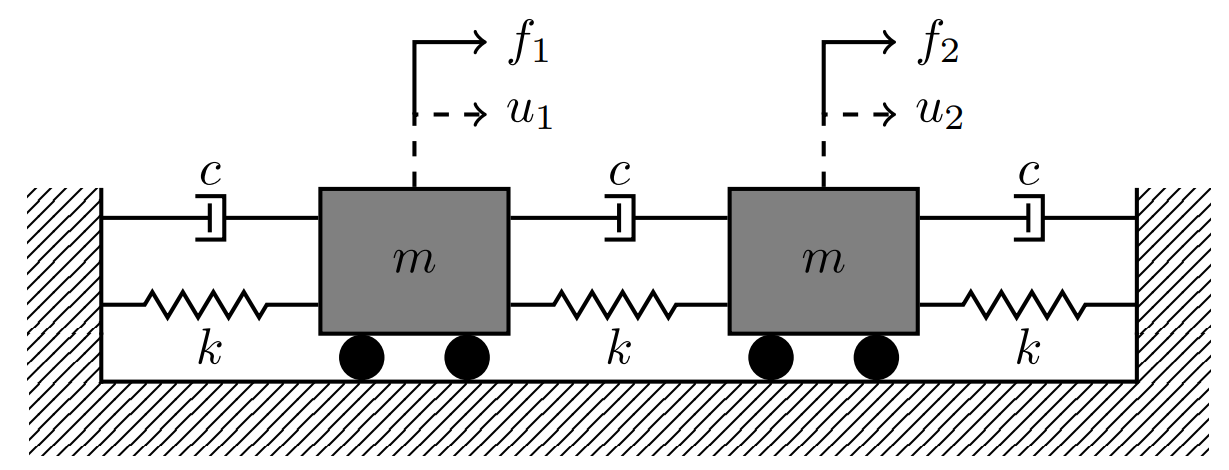
\includegraphics[width=.8\linewidth]{Slides/Figure/HeDaoDong.png}
                \caption{2 dofs system}
                \label{fig:placeholder}
            \end{figure}
        \end{column}
    
        \begin{column} {0.6\textwidth}
            \centering
            Phương trình động lực học:
            \begin{equation}\label{eq_PT2dofs_c}
                \begin{cases}
                    m \ddot{u}_1 + 2c\dot{u}_1 - c\dot{u}_2 + 2ku_1 - ku_2 = f_1 \\
                    m \ddot{u}_2 + 2c\dot{u}_2 - c\dot{u}_1 + 2ku_2 - ku_1 = f_2 \\
                \end{cases}
            \end{equation}
        \end{column}
    \end{columns}
    
    Biểu diễn dưới dạng ma trận:
    \begin{equation}\label{eq_PT2dofs_c_matrix}
        \underbrace{\begin{bmatrix}
            m & 0\\ 0 & m
        \end{bmatrix}}_{\bf M}\underbrace{\begin{bmatrix}
            \ddot{u}_1 \\ \ddot{u}_2
        \end{bmatrix}}_{\ddot{\bf u}} + \underbrace{\begin{bmatrix}
            2c & -c \\ -c & 2c
        \end{bmatrix}}_{\bf C}\underbrace{\begin{bmatrix}
            \dot{u}_1 \\ \dot{u}_2
        \end{bmatrix}}_{\dot{\bf u}} +\underbrace{\begin{bmatrix}
            2k & -k \\ -k & 2k
        \end{bmatrix}}_{\bf K} \underbrace{\begin{bmatrix}
            u_1 \\ u_2
        \end{bmatrix}}_{\bf u} = \underbrace{\begin{bmatrix}
            f_1 \\ f_2
        \end{bmatrix}}_{\bf f} 
    \end{equation}

    \textbf{PT tổng quát:}
        \begin{equation}\label{eq_PTmatrix}
            {\bf M}\ddot{\bf u} + {\bf C}\dot{\bf u} + {\bf K}{\bf u} = {\bf f}
        \end{equation}
\end{frame}

\subsection{Dao động tự do}
%% Slide %%
\begin{frame}{Dao động tự do - Không cản (c = 0, f1=f2=0)}

\vspace{7mm}

Các bậc tự do dao động với cùng sự phụ thuộc theo thời gian nên chúng ta có:
\begin{equation}
    {\bf u} = \begin{bmatrix}
        u_1 \\ u_2
    \end{bmatrix} = {\bf X}cos(\Omega t)
\end{equation}

Thay vào \ref{eq_PTmatrix} ta có:
\begin{equation}
    (\mathbf{K}-\Omega^2 \mathbf{M})\mathbf{X}=0
\end{equation}

Ta đưa về bài toán tìm trị riêng và vector riêng của ma trận. PT có nghiệm khác 0 khi:

\begin{equation}
    det(\mathbf{K}-\Omega^2 \mathbf{M}) = 0
\end{equation}

\end{frame}

%% Slide %%
\begin{frame}{Dao động tự do - Không cản (c = 0, f1=f2=0)}

Ta tìm được 2 giá trị của tần số riêng:
\begin{equation}
    \Omega^2 =  \Omega_1^2 = \frac{k}{m} \quad \hbox{và} \quad \Omega^2 = \Omega_2^2 = \frac{3k}{m}
\end{equation}
Vector riêng của hệ là:
\begin{equation}
    {\bf X} = {\bf X}_1 = \begin{bmatrix}
        1 \\ 1
    \end{bmatrix} \quad \hbox{và} \quad {\bf X} = {\bf X}_2 = \begin{bmatrix}
        1 \\ -1
    \end{bmatrix}
\end{equation}
Nghiệm tổng quát của hệ là:
\begin{equation}
    {\bf u}=\underbrace{\left(A_1 \cos \left(\Omega_1 t\right)+B_1 \sin \left(\Omega_1 t\right)\right) {\bf X}_1}_{\hbox{Mode 1}}+\underbrace{\left(A_2 \cos \left(\Omega_2 t\right)+B_2 \sin \left(\Omega_2 t\right)\right) {\bf X}_2}_{\hbox{Mode 2}}
\end{equation}  
\end{frame}

\subsection{Dao động cưỡng bức}

%% Slide %%
\begin{frame}{Dao động cưỡng bức - Không có giảm chấn (c=0, f1 $\neq$ 0, f2 $\neq$ 0)}

\vspace{5mm}

Xét trường hợp $f_1 = F_1\cos(\omega t)$ và $f_2 = F_2\cos(\omega t)$.

Đặt ${\bf f} = \begin{bmatrix} F_1 \\ F_2\end{bmatrix}\cos(\omega t) = {\bf F}\cos(\omega t)$ va ${\bf u} = \begin{bmatrix} U_1 \\ U_2\end{bmatrix}\cos(\omega t) = {\bf U}\cos(\omega t)$.

Thay vào phương trình \eqref{eq_PTmatrix} ta có:
\begin{equation}
    {\bf U} = (-\omega^2{\bf M}+{\bf K})^{-1} {\bf F}.
\end{equation}
Từ đó ta tính được $U_1$ và $U_2$:
\begin{equation}
     U_1 = \frac{F_1(2k-m\omega^2)+F_2k}{(k-m\omega^2)(3k-m\omega^2)} \quad \hbox{và} \quad U_2 = \frac{F_1k+F_2(2k-m\omega^2)}{(k-m\omega^2)(3k-m\omega^2)}
\end{equation}
\end{frame}

%% Slide %%
\begin{frame}{Dao động cưỡng bức - Có giảm chấn (c $\neq$ 0, f1 $\neq$ 0, f2 $\neq$ 0)}

\vspace{7mm}

Biểu diễn PT dưới dạng số phức. Đặt ${\bf f} = {\bf F}e^{j\omega t}$ va ${\bf u} = {\bf U}e^{j\omega t}$, từ đó tính được:

\begin{equation}
    {\bf U} = (-\omega^2{\bf M} + j\omega{\bf C} + {\bf K})^{-1} {\bf F}
\end{equation}

Ta có:

\begin{equation}\label{eq_nghiemphuc}
    \begin{aligned}
        {U}_1 &=\frac{\left(2 F_1+F_2\right) k-F_1 m \omega^2+j c\left(2 F_1+F_2\right) \omega}{\left(j c \omega+k-m \omega^2\right)\left(3 j c \omega+3 k-m \omega^2\right)}\\
        {U}_2 &=\frac{\left(F_1+2 F_2\right) k-F_2 m \omega^2+j c\left(F_1+2 F_2\right) \omega}{\left(j c \omega+k-m \omega^2\right)\left(3 j c \omega+3 k-m \omega^2\right)}
    \end{aligned}
\end{equation}
\end{frame}

%% Slide %%
\begin{frame}{Dao động cưỡng bức - Có giảm chấn (c $\neq$ 0, f1 $\neq$ 0, f2 $\neq$ 0)}

\vspace{10mm}

Biên độ của $U_1$ và $U_2$:

\begin{equation}
    \begin{aligned}
         \left|U_1\right|&=\frac{\sqrt{\left(2 c F_1 \omega+c F_2 \omega\right)^2+\left(2 F_1 k+F_2 k-F_1 m \omega^2\right)^2}}{\sqrt{c^2 \omega^2+\left(k-m \omega^2\right)^2} \sqrt{9 c^2 \omega^2+\left(m \omega^2-3 k\right)^2}} \\
         \left|U_2\right|&=\frac{\sqrt{\left(c F_1 \omega+2 c F_2 \omega\right)^2+\left(F_1 k+2 F_2 k-F_2 m \omega^2\right)^2}}{\sqrt{c^2 \omega^2+\left(k-m \omega^2\right)^2} \sqrt{9 c^2 \omega^2+\left(m \omega^2-3 k\right)^2}}\\
    \end{aligned}
\end{equation}
\end{frame}

\subsection{Giải PT dao động tổng quát}

%% Slide %%
\begin{frame}{Phương pháp Runge-Kutta}

Miền tích phân thời gian sẽ được rời rạc hóa thành các bước thời gian: $t_0, t_1, t_2, t_3, t_4, \dots, t_n$ với $\Delta t = (t_n-t_0)/n$

Phương pháp Runge-Kutta được sử dụng để giải phương trình đạo hàm bậc nhất : $\frac{d {\bf u}}{d t}={\bf f}(t,{\bf u}) ,\quad {\bf u}\left(t_0\right)={\bf u}_0$

\begin{equation}
    {\bf u}_{n+1} = {\bf u}_n + h \sum_{i=1}^s b_i {\bf k}_i
\end{equation}

\begin{equation}
\begin{aligned}
     {\bf k}_1 & = {\bf f}(t_n, {\bf u}_n), \\
     {\bf k}_2 & = {\bf f}(t_n+c_2h, {\bf u}_n+h(a_{21}{\bf k}_1)), \\
     {\bf k}_3 & = {\bf f}(t_n+c_3h, {\bf u}_n+h(a_{31}{\bf k}_1+a_{32}{\bf k}_2)), \\
         & \ \ \vdots \\
     {\bf k}_s & = {\bf f}(t_n+c_sh, {\bf u}_n+h(a_{s1}{\bf k}_1+a_{s2}{\bf k}_2+\cdots+a_{s,s-1}{\bf k}_{s-1})).
\end{aligned}
\end{equation}

\end{frame}

%% Slide %%
\begin{frame}{Phương pháp Runge-Kutta}
Ma trận Butcher
\begin{equation}
\begin{array}{c|cccc}
0      &        &        &        &        \\
c_{2}  & a_{21} &        &        &        \\
c_{3}  & a_{31} & a_{32} &        &        \\
\vdots & \vdots & \vdots & \ddots &        \\
c_{s}  & a_{s1} & a_{s2} & \cdots & a_{s,s-1} \\
\hline
       & b_{1}  & b_{2}  & \cdots & b_{s}
\end{array}   
\end{equation}

\begin{columns}
    \begin{column}{0.23\textwidth}
        Runge-Kutta bậc 2
        \vspace{-3mm}
        \begin{equation*}
         \begin{array}{c|cccc}
        0 & & \\
        1/2 & 1/2 & \\
        \hline
         & 0 & 1
        \end{array}   
        \end{equation*}
    \end{column}
    
    \begin{column}{0.38\textwidth}
        Runge-Kutta bậc 4 (RK4)
        \vspace{-3mm}
        \begin{equation*}
        \begin{array}{c|cccc}
        0 & & & & \\
        1/2 & 1/2 & & & \\
        1/2 & 0 & 1/2 & & \\
        1 & 0 & 0 & 1 &\\
        \hline
         & 1/6 & 1/3 & 1/3 & 1/6
        \end{array}   
        \end{equation*}
    \end{column}

    \begin{column}{0.38\textwidth}
        Runge-Kutta 3/8
        \vspace{-3mm}
        \begin{equation*}
        \begin{array}{c|cccc}
        0 & & & & \\
        1/3 & 1/3 & & & \\
        2/3 & -1/3 & 1 & & \\
        1 & 1 & -1 & 1 &\\
        \hline
         & 1/8 & 3/8 & 3/8 & 1/8
        \end{array}   
        \end{equation*}
    \end{column}
\end{columns}

\end{frame}

%% Slide %%
\begin{frame}{Phương pháp Runge-Kutta}

\textbf{Áp dụng:}

PT \ref{eq_PTmatrix} là 1 phương trình đạo hàm bậc 2. Để sử dụng thuật toán Runge-Kutta, chúng ta cần thực hiện đổi biến để đưa PT \ref{eq_PTmatrix} về đạo hàm bậc nhất.

Đặt ${\bf u}_1 = {\bf u}$ và ${\bf u}_2 = \dot{\bf u}$. Ta có: $\dot{\bf u}_1 = \dot{\bf u}$ va $\dot{\bf u}_2 = \ddot{\bf u}$.

\begin{equation}
    \begin{aligned}
    &\begin{cases}
        \dot{\bf u}_1 &= {\bf u}_2 \\
        \dot{\bf u}_2 &= {\bf M}^{-1}\left(-{\bf K}{\bf u}_1-{\bf C}{\bf u}_2 + {\bf f}\right)
    \end{cases} \\
    \Rightarrow &\begin{bmatrix}
        \dot{\bf u}_1 \\ \dot{\bf u}_2
    \end{bmatrix} = \begin{bmatrix}
        {\bf O} & {\bf I} \\
        -{\bf M}^{-1}{\bf K} & -{\bf M}^{-1}{\bf C}
    \end{bmatrix}\begin{bmatrix}
        {\bf u}_1 \\ {\bf u}_2
    \end{bmatrix} + \begin{bmatrix}
        {\bf O} \\ {\bf M}^{-1}{\bf f}
    \end{bmatrix} \\
    \Leftrightarrow & \dot{\bf U} = {\bf A} {\bf U} + {\bf B}
    \end{aligned}
\end{equation}

Trên python, phương pháp RK4 có sẵn trong thư viện \textbf{scipy.integrate}. Để sử dụng chúng ta dùng hàm \textbf{odeint}
    
\end{frame}

%% Slide %%
\begin{frame}{Phương pháp Newmark}

Phương pháp Newmark xấp xỉ các đạo hàm bậc nhất và bậc hai như sau:
\begin{equation}\label{eq_newmark}
    \begin{aligned}
    \dot{\bf u}_{n+1} &\approx \dot{\bf u}_n+(1-\gamma) \Delta t \ddot{\bf u}_n+\gamma \Delta t \ddot{\bf u}_{n+1}\\
    {\bf u}_{n+1} &\approx {\bf u}_n+\Delta t \dot{\bf u}_n+\left(1/2-\beta\right)(\Delta t)^2 \ddot{\bf u}_n+\beta(\Delta t)^2 \ddot{\bf u}_{n+1}
\end{aligned}
\end{equation}

$(\gamma, \beta)$ là các tham số Newmark. Một vài giá trị thường được sử dụng là $(1/2, 1/4)$, $(1/2, 1/6)$, $(1/2, 0)$.

Thay các xấp xỉ \ref{eq_newmark} vào PT \ref{eq_PTmatrix}:
\begin{equation}
\begin{aligned}
    \ddot{\bf u}_{n+1}={\bf S}^{-1}\left[{\bf f}_{n+1}-[{\bf C}\left(\dot{\bf u}_n\right.\right. & \left.+(1-\gamma) \Delta t \ddot{\bf u}_n\right) \\
& \left.-{\bf K}\left({\bf u}_n+\Delta t \dot{\bf u}_n+\left(1/2-\beta\right)(\Delta t)^2 \ddot{\bf u}_n\right)\right]
\end{aligned}
\end{equation}
Với ${\bf S} = {\bf M} + {\bf C}\gamma\Delta t + {\bf K}\beta(\Delta t)^2$.
    
\end{frame}

%% Slide %%
\begin{frame}{Phương pháp Newmark}
\vspace{15mm}
\textbf{Áp dụng:}
\begin{itemize}
    \item Xác định $\Delta t$, các tham số Newmark $(\gamma,\beta)$ và ma trận ${\bf S}$,
    \item Tại $t_0$, xác định vector ${\bf f}_0 = {\bf f}(t_0)$ và các điều kiện ban đầu của hệ (${\bf u}_0$ va $\dot{\bf u}_0$),
    \item Tinh $\ddot{\bf u}_0$ theo công thức $\ddot{\bf u}_0 = {\bf M}^{-1}\left({\bf f}_0 - {\bf C}\dot{\bf u}_0 - {\bf K}{\bf u}_0\right)$,
    \item Với mỗi $t_0, t_1, t_2, \dots,t_n$. Xác định ${\bf f}_{n+1}$ và tính $\ddot{\bf u}_{n+1}$ va ${\bf u}_{n+1}, \dot{\bf u}_{n+1}$ theo các công thức Newmark.
\end{itemize}
    
\end{frame}

%%%% Section2 %%%%

\section{Phương pháp số trong mô phỏng}
\subsection{Ví dụ}
%% Slide %%
\begin{frame}{Ví dụ}
PT Poisson:
\begin{equation}\label{eq_PTpoisson}
    \begin{aligned}
        -\frac{\partial^2u}{\partial x^2} &= x \quad x \in \left(0, 1\right) \\
        u\left(0\right) &= 2 \quad \left(\hbox{điều kiện biên Dirichlet}\right) \\
        \frac{\partial u}{\partial x} \left(1\right) &= 1 \quad \left(\hbox{điều kiện biên Neumann}\right) \\
    \end{aligned}
\end{equation}
Nghiệm chính xác của nó là:\begin{equation}\label{eq_sol}
    u\left(x\right) = \frac{-x^3 + 9x + 12}{6}
\end{equation}
Ta sẽ áp dụng các phương pháp số để giải phương trình đó và so sánh với nghiệm chính xác của nó.
\end{frame}

\subsection{Phương trình vi phân - Phương trình dạng mạnh và dạng yếu}

%% Slide %%
\begin{frame}{Phương trình vi phân - Phương trình dạng mạnh}
\vspace{12mm}
Dạng mạnh chính là dạng biểu diễn của phương trình vi phân. Nghiệm của phương trình thỏa mãn với mọi điểm trong miền xác định.

 \begin{equation}
    \begin{aligned}
        -\frac{\partial^2u}{\partial x^2} &= x \quad x \in \left(0, 1\right) \\
        u\left(0\right) &= 2 \quad \left(\hbox{điều kiện biên Dirichlet}\right) \\
        \frac{\partial u}{\partial x} \left(1\right) &= 1 \quad \left(\hbox{điều kiện biên Neumann}\right) \\
    \end{aligned}
\end{equation}
\end{frame}

%% Slide %%
\begin{frame}{Phương trình vi phân - Phương trình dạng yếu}

Được biểu diễn dưới dạng tích phân của tích phương trình dạng mạnh với một hàm thử trên miền xác định. 

PP Ritz-Galerkin: xấp xỉ nghiệm $u$ của PT Poisson bằng 1 nghiệm $u^h$.
\begin{equation}
    R_{\Omega} = -\frac{\partial^2 u^h}{\partial x^2} - x \neq 0 \quad x \in \left(0, 1\right) \; \hbox{va} \;
    R_{\partial\Omega} = \frac{\partial u^h}{\partial x} \left(1\right) - 1 \neq 0
\end{equation}

Gọi $v$ là hàm thử:
\begin{equation}\label{eq_Ritz}
    \int_0^1 v R_{\Omega}dx + v(1)R_{\partial\Omega} = 0 
    \Rightarrow \int_0^1 v \left(-\frac{\partial^2 u^h}{\partial x^2} - x\right)dx + v(1)\left(\frac{\partial u^h}{\partial x} \left(1\right) - 1\right) =0
\end{equation}

\begin{equation}\label{eq_weakform}
    \Rightarrow \int_0^1 \frac{\partial u^h}{\partial x} \frac{\partial v}{\partial x}dx - v(1) - \int_0^1 v x dx =0
\end{equation}

\end{frame}


\subsection{Phương pháp số - Phương pháp sai phân hữu hạn và phần tử hữu hạn}

%% Slide %%
\begin{frame}{Phương pháp số - Phương pháp sai phân hữu hạn}

Phương pháp sai phân hữu hạn giải trực tiếp PT dạng mạnh

Chuỗi Taylor:
\begin{equation}\label{eq_taylor}
    \begin{aligned}
        f(x+h) &=f(x)+f^{\prime}(x) h+\frac{f^{\prime \prime}(x)}{2!} h^2+\frac{f^{\prime \prime \prime}(x)}{3!} h^3+\frac{f^{(4)}\left(\xi_1\right)}{4!} h^4 + \dots\\
        f(x-h) &=f(x)-f^{\prime}(x) h+\frac{f^{\prime \prime}(x)}{2!} h^2-\frac{f^{\prime \prime \prime}(x)}{3!} h^3+\frac{f^{(4)}\left(\xi_2\right)}{4!} h^4 + \dots
\end{aligned}
\end{equation}
Từ đây ta có các cách để xấp xỉ đạo hàm bậc nhất:
\begin{equation}\label{eq_bac1}
    \begin{aligned}
        f^{\prime}(x) &\approx \frac{f(x+h) - f(x)}{h} \quad \hbox{sai phân tiến} \\
        f^{\prime}(x) &\approx \frac{f(x) - f(x-h)}{h} \quad \hbox{sai phân lùi} \\
        f^{\prime}(x) &\approx \frac{f(x+h) - f(x-h)}{2h} \quad \hbox{sai phân trung tâm} \\
    \end{aligned}
\end{equation}
\end{frame}

%% Slide %%
\begin{frame}{Phương pháp số - Phương pháp sai phân hữu hạn}
\vspace{7mm}
Tương tự, ta có thể xấp xỉ đạo hàm bậc 2:
\begin{equation}\label{eq_bac2}
    f^{\prime \prime}(x) \approx \frac{f(x+h) -2f(x) + f(x-h)}{h^2}
\end{equation}
Áp dụng cho bài toán ví dụ: Giả sử ta chia miền $x \in (0, 1)$ thành $N=3$ điểm cách đều nhau. Theo công thức sai phân ta có:
\begin{equation}
    - \frac{u_1 - 2u_2 +u_3}{h^2} = x_2
\end{equation}
\begin{equation}
    \frac{u_3 -u_2}{h} = 1
\end{equation}
\end{frame}

%% Slide %%
\begin{frame}{Phương pháp số - Phương pháp sai phân hữu hạn}

Kết hợp với điều kiện biên Dirichlet, ta có hệ phương trình:

\begin{equation}
    \left\{\begin{matrix}
        &u_1 & & &=2 \\
        &u_1/h^2 &-2u_2/h^2 &+ u_3/h^2 &=-x_2 \\
        & &-u_2/h &+ u_3/h &= 1\\
    \end{matrix}\right.
\end{equation}

Viết dưới dạng ma trận
\begin{equation}
    \begin{bmatrix}
        1 & 0 & 0 \\ 1/h^2 & -2/h^2 & 1/h^2 \\ 0 & -1/h & 1/h 
    \end{bmatrix}\begin{bmatrix}
        u_1 \\ u_2 \\ u_3 
    \end{bmatrix} = \begin{bmatrix}
        2 \\ x_2 \\ 1
    \end{bmatrix}
\end{equation}
Giải phương trình trên ta sẽ tính được giá trị các nút.
\end{frame}

%% Slide %%
\begin{frame}{Phương pháp số - Phương pháp sai phân hữu hạn}

\vspace{7mm}
Nghiệm của PT, giải bằng phương pháp sai phân hữu hạn với $N=3$, $N=10$ và $N=100$:
\begin{figure}[htbp]
    \centering
    \begin{subfigure}[b]{0.3\linewidth}
        \centering
        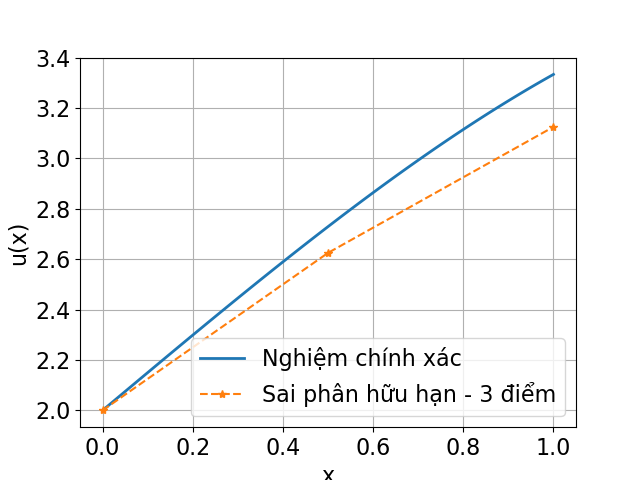
\includegraphics[width=\linewidth]{Slides/Figure/SPHH_3p.png}
        \caption{3 nút}
        \label{fig:SPHH_3p}
    \end{subfigure}\hfill
    \begin{subfigure}[b]{0.3\linewidth}
        \centering
        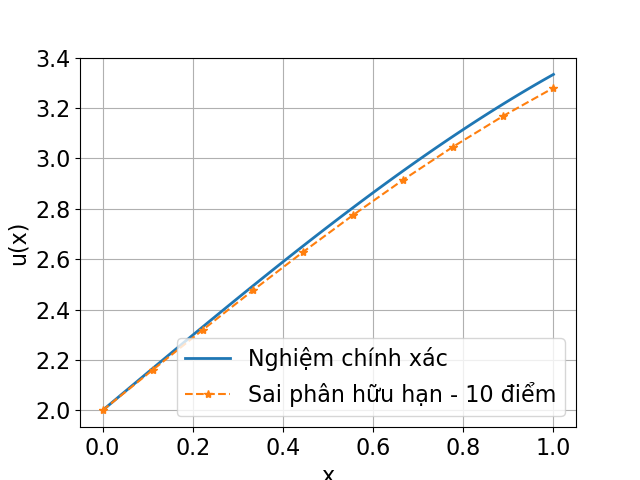
\includegraphics[width=\linewidth]{Slides/Figure/SPHH_10p.png}
        \caption{10 nút}
        \label{fig:SPHH_10p}
    \end{subfigure}\hfill
    \begin{subfigure}[b]{0.3\linewidth}
        \centering
        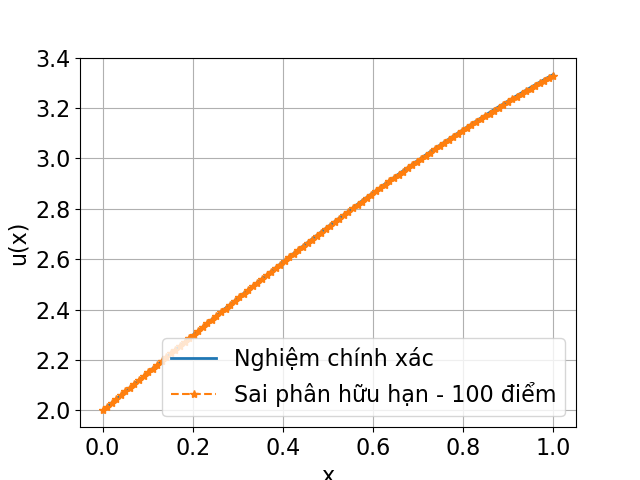
\includegraphics[width=\linewidth]{Slides/Figure/SPHH_100p.png}
        \caption{100 nút}
        \label{fig:SPHH_100p}
    \end{subfigure}
    \label{fig_SPHHresults}
\end{figure}
\end{frame}

%% Slide %%
\begin{frame}{Phương pháp số - Phương pháp phần tử hữu hạn}

\vspace{7mm}

Phương pháp phần tử hữu hạn giải trực tiếp PT dạng yếu \ref{eq_weakform}

Chia miền xác định thành các miền con $\Omega_e$ không giao nhau gọi là các phần tử (chia lưới)
\begin{figure}[htbp]
    \centering
    \begin{subfigure}[b]{0.45\linewidth}
        \centering
        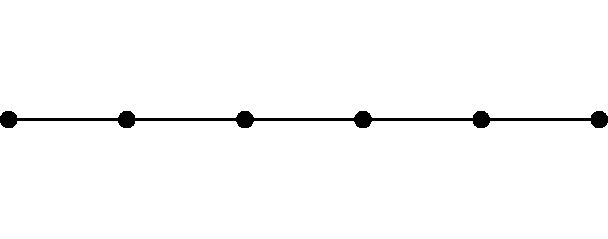
\includegraphics[width=\linewidth]{Slides/Figure/FEM1D.pdf}
        \caption{1D}
    \end{subfigure}\hfill
    \begin{subfigure}[b]{0.45\linewidth}
        \centering
        
\includegraphics[width=\linewidth]{Slides/Figure/FEM2D.pdf}
        \caption{2D}
    \end{subfigure}
\end{figure}
\end{frame}

%% Slide %%
\begin{frame}{Phương pháp số - Phương pháp phần tử hữu hạn}

\vspace{3mm}
$\bullet$ Xấp xỉ nghiệm $u^h(x)$
\begin{equation}\label{eq_interpolation}
    u^h(x) = \sum\limits_{i=1}^n N_i(x) u_i = \underbrace{\begin{bmatrix}
        N_1(x) \dots N_n(x)
    \end{bmatrix}}_{{\bf N}(x)} \underbrace{\begin{bmatrix}
        u_1 \\ \vdots \\ u_n 
    \end{bmatrix}}_{\bf u}
\end{equation}

Hàm thử $v$ sẽ được chọn sao cho nó có cùng hàm nội suy với nghiệm xấp xỉ $u^h$ (nguyên lý Bubnov-Galerkin)
\begin{equation}\label{eq_interpolation_test}
    v(x) = \sum\limits_{i=1}^n N_i(x) v_i = {{\bf N}(x)}{\bf v}
\end{equation}
\end{frame}

%% Slide %%
\begin{frame}{Phương pháp số - Phương pháp phần tử hữu hạn}

\vspace{10mm}

Thay các xấp xỉ này vào PT \ref{eq_weakform}:
\begin{equation}\label{eq_matrixform}
    \underbrace{\left(\int\limits_0^1\left(\frac{\partial{\bf N}}{\partial x}\right)^T\frac{\partial{\bf N}}{\partial x} dx\right)}_{\bf K}{\bf u} = \underbrace{[{\bf N}(1)]^T + \int\limits_0^1 [{\bf N}(x)]^Tx dx}_{\bf F} 
\end{equation}

Giải PT trên:

\begin{equation}
    \Rightarrow {\bf u} = {\bf K}^{-1}{\bf F}
\end{equation}
\end{frame}

%% Slide %%
\begin{frame}{Phương pháp số - Phương pháp phần tử hữu hạn}

$\bullet$ Hàm nội suy ${\bf N}(x)$

Hàm đa thức thỏa mãn tính chất $N_i(x_i) = 1$ và $N_i(x_j) = 0$ với $j \neq i$

Xét trường hợp 1D:
\begin{equation}\label{eq_shape1D}
    \begin{aligned}
        N_1(x) &= \frac{1}{x_2-x_1}\left(x_2-x\right) \\
        N_2(x) &= \frac{1}{x_2-x_1}\left(x-x_1\right) \\
    \end{aligned}
\end{equation}

\begin{figure}
    \centering
    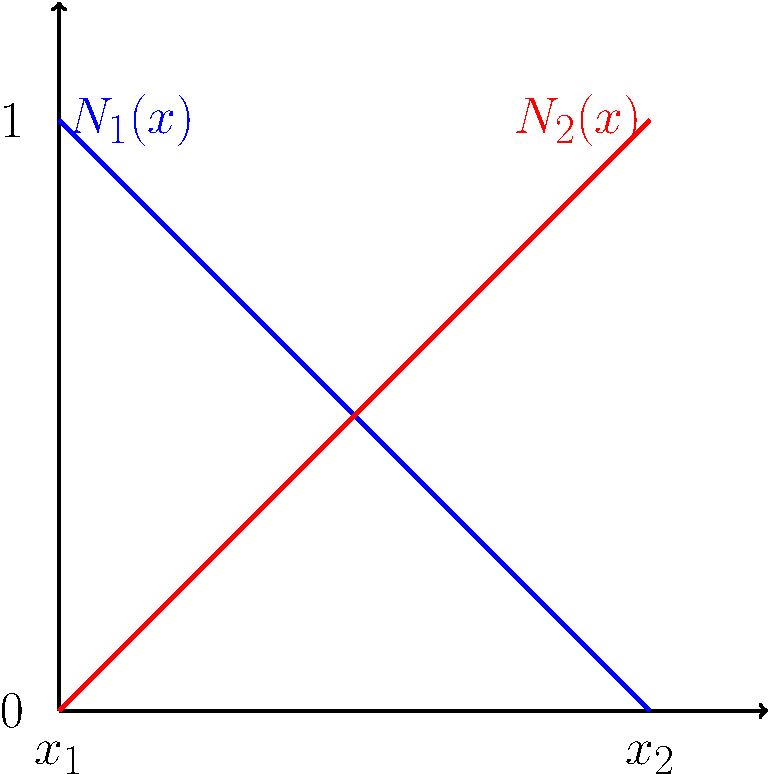
\includegraphics[width=0.16\linewidth]{Slides/Figure/shape_func.pdf}
    \caption{Hàm nội suy 1D, tuyến tính}
\end{figure}

\end{frame}

%% Slide %%
\begin{frame}{Phương pháp số - Phương pháp phần tử hữu hạn}
\vspace{3mm}
$\bullet$ Lắp ghép các phần tử

Xét với trường hợp miền xác định 1D được chia thành 2 phần tử $e1$ và $e2$. Áp dụng các phương trình trên, ta xác định được ma trận ${\bf K}^{e1}$, ${\bf K}^{e2}$ và các vector ${\bf F}^{e1}$, ${\bf F}^{e2}$ tương ứng với mỗi phần tử.

${\bf u} = [u_1 \; u_2 \; u_3]^T$: vector bậc tự do của các nút.

Lưu ý rằng: $u_2 = u_2^{e1} + u_1^{e2}$. Hệ ma trận cho vector ${\bf u}$ được viết lại như sau

\begin{equation}
    \begin{bmatrix}
        K_{11}^{e1} & K_{12}^{e1} & 0\\
        K_{21}^{e1} & K_{22}^{e1}+K_{22}^{e2} & K_{23}^{e2} \\
        0 & K_{32}^{e2} & K_{33}^{e2}
    \end{bmatrix}\begin{bmatrix}
        u_1 \\ u_2 \\ u_3
    \end{bmatrix} = \begin{bmatrix}
        0 \\ 0 \\ 1
    \end{bmatrix} + \begin{bmatrix}
        F_1^{e1} \\ F_2^{e1}+F_2^{e2} \\ F_3^{e2}
    \end{bmatrix}
\end{equation}

\textbf{ Kết hợp với điều kiện biên Dirichlet và giải PT trên}, ta thu được giá trị của ${\bf u}$.
\cite{golub2013matrix}
\end{frame}

%% Slide %%
\begin{frame}{Phương pháp số - Phương pháp phần tử hữu hạn}
\vspace{10mm}
Nghiệm của PT, giải bằng phương pháp phần tử hữu hạn với $2$, $10$ và $100$ phần tử:

\begin{figure}[htbp]
    \centering
    \begin{subfigure}[b]{0.3\linewidth}
        \centering
        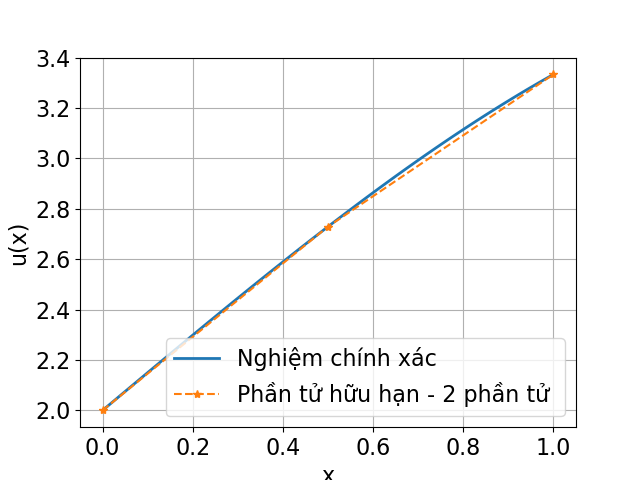
\includegraphics[width=\linewidth]{Slides/Figure/PTHH_2el.png}
        \caption{2 phần tử}
    \end{subfigure}\hfill
    \begin{subfigure}[b]{0.3\linewidth}
        \centering
        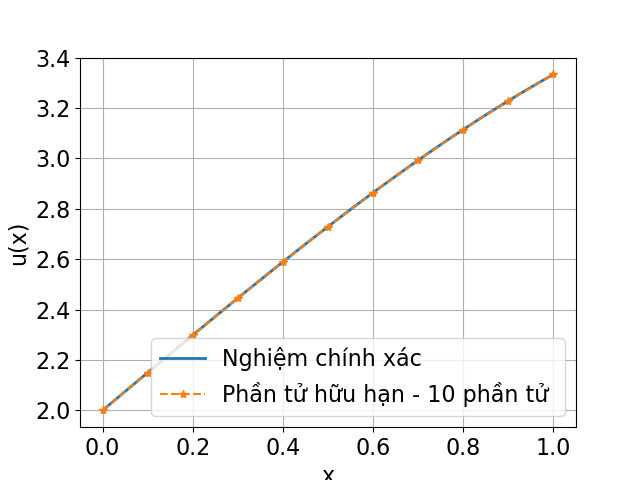
\includegraphics[width=\linewidth]{Slides/Figure/PTHH_10el.png}
        \caption{10 phần tử}
    \end{subfigure}\hfill
    \begin{subfigure}[b]{0.3\linewidth}
        \centering
        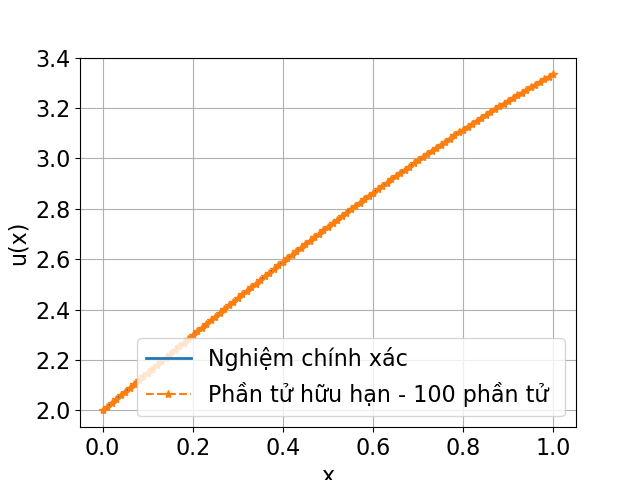
\includegraphics[width=\linewidth]{Slides/Figure/PTHH_100el.png}
        \caption{100 phần tử}
    \end{subfigure}
\end{figure}
\end{frame}

%% Slide %%
\begin{frame}[allowframebreaks]{Tài liệu tham khảo}
    \nocite{*}
    \printbibliography
\end{frame}

\end{document}